\subsection{Previous Methods.}

We adapt the methods to generate a  word distribution for each test document, and output the $s$ most likely unseen words according to this distribution.

\begin{itemize}

\item
{\bf Baseline:} The word distribution for every test document is the distribution over words in the training set. 

\item
{\bf KNN:} KNN finds the $k$ most similar training documents to a
testing document, where similarity is defined as the cosine between
the two documents as vectors in the word space. For a testing
document, KNN uses the distribution over words in
its $k$ closest training documents to predict. Notice baseline is just KNN with
$k$ equal to the number of training documents.


\item
{\bf LDA:} It is $NP$-hard to find the maximum likelihood fit to the LDA model,
so in practice, the prevailing approach to learn LDA model is local
search. We adopted the algorithm implemented by Blei \cite{LDAcode}
using variational EM (see \cite{Blei2003a}).

The LDA algorithm has two procedures,{\em "estimation"} and {\em "inference"}. {\em "estimation"} takes a collection of documents as
input, and outputs estimated model parameters for the corpus, in
particular the estimated term-topic matrix. {\em "inference'} takes a
collection of documents as well as a LDA model, and outputs an
inferred topic mixture for each document. For our prediction task, we
use the estimated term-topic matrix of the training set and the topic
mixture for each testing document to estimate the most likely unseen
words.

\item
{\bf LDA(MALLET)} We also experiment with another implementation of LDA in Mallet \cite{McCallumMALLET} using fast Gibbs sampling \cite{MimnoSparse}. The implementation in Mallet follows a similar {\em "estimation"} and {\em "inference"} workflow.


\item {\bf LDAT, LDAC} For generated LDA datasets, we have two
  "cheating" algorithms as benchmarks. LDAT knows the real term-topic
  matrix $A$ of the model and uses the {\em "inference"} routine to find a
  word distribution for each document.  LDAC knows the real
  term-document matrix $M$ for each testing document, and uses the
  real word distribution for a test document.  LDAC is the best we can
  do given sampling noise.

\item
{\bf K-means:} We partition the training documents using $k$-means, with $1-\cos(w,w')$ as the distance between documents $w$ and $w'$.
We use the $k$ cluster centers as the term-topic matrix, and uses the {\em "inference"} procedure of BLei's LDA implementation to produce a word
distibution for each test document. 

\item {\bf LSI}.  We compute the best rank-$k$ subspace approximation of the document-word
matrix for the training set. For each test document, we project it onto the subspace, and get a word distribution by shifting and normalizing its projection. 

\end{itemize}

%% \subsection{LSI}
%% In the LDA model, we have $M=AW$, where $A$ and $W$ are the word-topic matrix and topic-document matrix respectively. Each column of M is a probability distribution on words. The $i$th document we observe is a set of i.i.d samples from the distribution $M_i$, and we have the observed word distribution $\hat{M}_i$. In the word space $\mathbb{R}^m$, all colunms of $M$ lie in the $k$-dimensional subspace spanned by the $k$ topics $A$. The sampled document $\hat{M}_i$ will be a noisy version of $M_i$, so in the word space $\mathbb{R}^m$, the points in $\hat{M}$ will be scattered close to the subspace of $A$.

%% LSI works by computing the best rank $k$ approximation to $\hat{M}$ of the training documents
%% \begin{align*}
%% &min_{U,\Sigma,V}\norm{\hat{M}-U\Sigma V}_F\\
%% \text{such that } &U\in \mathbb{R}^{m\times k},V\in \mathbb{R}^{k\times n}\text{  } orthonormal, \Sigma\in \mathbb{R}^{k\times k}\text{ }diagonal.
%% \end{align*}
%% The optimal $U,S,V$ are computed using singular value decomposition
%% (SVD) of $\hat{M}$. LSI is not a statistical model in that the $U$ and
%% $V$ matrices contain negative entries. The subspace spanned by columns
%% of $U$ serve as an approximation of the subspace of $A$. Notice if we
%% carry out SVD on $M$, the subspace of $U$ will be exactly the same as
%% subspace of $A$.\footnote{This assumes that $k$ is the number of
%%   topics used in the LDA model which generated the data. This $k$ is
%%   provided to all algorithms. For generated data, this parameter is
%%   easy to recover in any case.} For a testing document $w$, we find
%% its projection $\hat{w}=UU^Tw$ on the subspace of $U$, and predict $s$
%% unseen words with largest entries in $\hat{w}$.

\subsection{Projector}

Projector is our new algorithm that builds upon LSI, and reconstructs
a term-topic probability matrix $\hat{A}$. The motivation is that SVD
is computationally more efficient than the LDA algorithm, and has a
clear geometric interpretation, but doesn't recover the topics as
distributions of words. We aim to start from the subspace computed by
SVD, and use some straightforward operation to construct the
topics. The algorithm is as
follows
\begin{description}
	\item[Input] $\hat{M}$: observed distributions of training documents, $k$: number of topics, $\delta$: algorithm parameter
	\item[Shift] Shift the training documents to be centered at the origin.\\
			     $center=\frac{1}{n}\sum_{i=1}^n\hat{M}_i$\\
			     $\hat{M}_i=\hat{M}_i-center\qquad \forall i=1,\ldots,n$
	\item[SVD] Compute the U, the best rank $(k-1)$-dimension approximation to the column space of $\hat{M}$\\
                                 Project all $\hat{M}_i$'s to the subspace $U$, denote $V_i$ as the projections.
	\item[Clustering] Use k-means to cluster the $V_i$'s into $k$ clusters, where in the k-means algorithm the distance between two points $x,y$ is defined as $1-cos(x,y)$.\\
				      Let $C_1,\ldots,C_k$ be the centers of the $k$ clusters (center in the sense as in euclidean distance).
	\item[Scale] Scale $C_1,\ldots,C_k$ by the smallest common scalar so that $\delta n$ of $V_1,\ldots,V_n$ are contained in the hull with $C_1,\ldots,C_k$ as vertices. 
	\item[Whitening] Make all $C_i$ distribution over words: Map all the $C_i$'s to the original word space, and then set $C_i=C_i+center$, truncate the negative entries in $C_i$ to be $0$, normalize $C_i$ so the sum of entries is $1$.\\
                                            Return $\hat{A}_i=C_i$ be the recovered topics.
\end{description}
We illustrate in figure~\ref{fig:projectorVis} how our algorithm works
using the a visualization on two datasets with $k=3$
topics.


The design of our algorithm is based on geometric intuitions of the documents
as points in the high dimensional word space. With LDA as the underlying generative model, if we consider each document as its true underlying distribution over words without the sampling noise, they reside in the $(k-1)$-simplex subspace with the $k$ topics as vertices. Our {\em Shift} and {\em SVD} steps aim to approximatley find this $(k-1)$-dimensional subspace.

After projecting all documents onto the subspace, the projected points lie approximately inside the convex hull of the $k$ topics. The origin also lies inside the convex hull, and the $k$ topics are along the pointy directions. We heuristically find the pointy directions using $k$-means with distances defined based on cosine similarity. 

Documents are convex combinations of the topics. The more interior points have more balanced weights on a relatively large number of topics, while points further away from the origin have large portion from a few topics, and the vertices are pure topics. The {\em Scale} step exploits this intuition by starting from the cluster centers, which gives the pointy directions, and pushing the centers away from the origin to find a convex hull approximately contains all the documents. As long as there is a slightly stronger presence of one topic in a cluster center, the scaling will amplify this topic. Finally we do some post processing to get valid distributions over words using the corners. 
\begin{figure}[h]  
   \begin{center}

        \subfigure[$\alpha=0.1,\beta=0.25,k=3$]{

            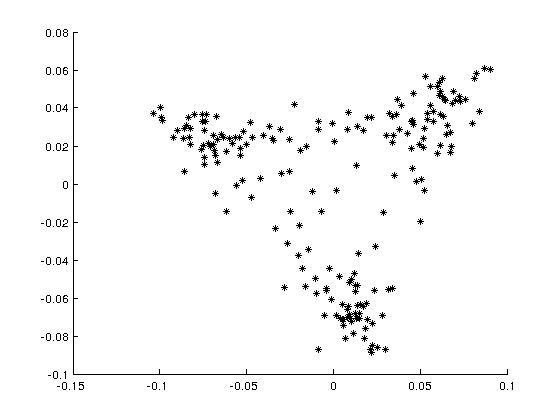
\includegraphics[width=0.35\textwidth]{c1.jpg}
        }
        \subfigure[Algorithm illustration with $\delta=0.8$]{

           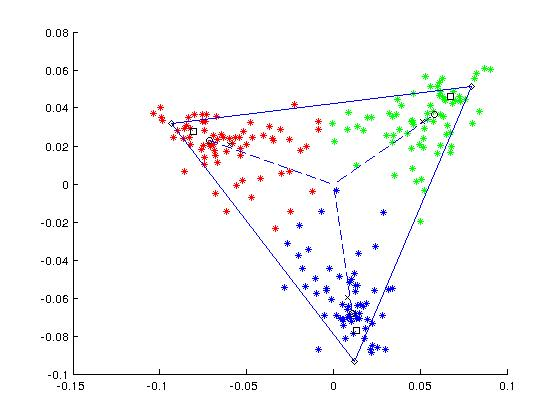
\includegraphics[width=0.35\textwidth]{c2.jpg}
        }\\ 
        \subfigure[$\alpha=0.8,\beta=0.25,k=3$]{

            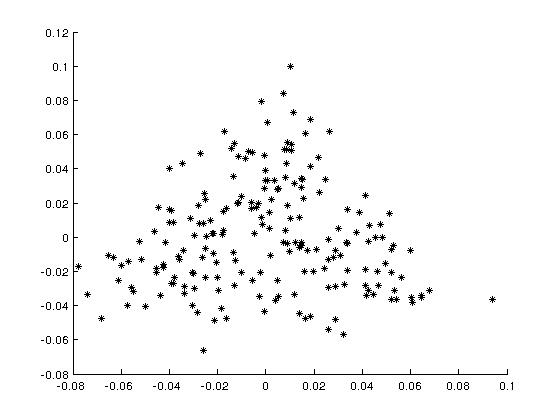
\includegraphics[width=0.35\textwidth]{b1.jpg}
        }
        \subfigure[Algorithm illustration with $\delta=0.8$]{

            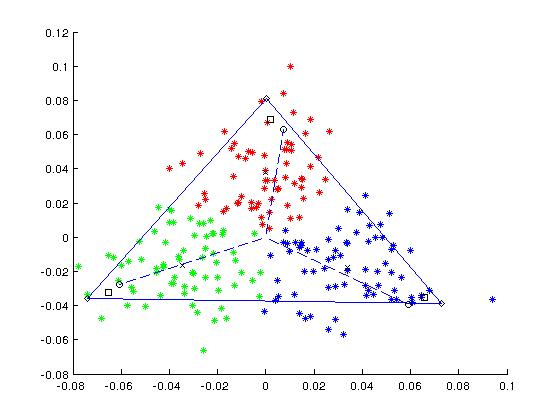
\includegraphics[width=0.35\textwidth]{b2.jpg}
        }

    \end{center}
    \caption{Illustration of Projector. The left figures are the $V_i$'s after the SVD step. In the right figures, the black 'o's at the ends of dotted lines are the real topic, black $\times$ are the $C_i$'s before scaling, black $\diamond$ are $C_i$'s after scaling, and black $\Box$ are the recovered $\hat{A}_i$'s. All points in the plot are after shifting and projected on the SVD subspace. }
\label{fig:projectorVis}
\end{figure}


We use estimated $\hat{A}$ and the inference procedure of the LDA
algorithm to predict words for testing documents. We use the inference
procedure of LDA since LDAT also uses it, so we can attribute
the performance difference between LDAT and Projector to the quality
of $\hat{A}$ compared to the real topics.

We also experimented with a version of projector which does
not use LSI as a first step; it just proceeds
with $k$-means, then we project the documents into the subspace
that contains the means and scale as above.  The results
were quite similar to the results above so we do not
include them here. 

%% \subsection{Projector with $k$-means}

%% We run 
